%========================================================================================
% TU Dortmund, Informatik Lehrstuhl VII
%========================================================================================
\chapter{Spiel}
\label{Spiel}
%
In diesem Abschnitt wird das Snake Spiel beschrieben und die Funktionen von Elementen im Gameplay oder Buttons erkl{\"a}rt. Dabei wird gar nicht auf die Implementierung eingegangen, sondern nur erkl{\"a}rt wie das Spiel funktioniert.


\section{Spiel - Hauptmen{\"u}}
\label{Spiel_-_Hauptmenü}
%
\begin{figure}[h]
 \centering
 \includegraphics[scale=0.5]{bilder/Hauptmenü}
 \caption{Hauptmen{\"u}}
 \label{fig:hauptmenü}
\end{figure}
Das Hauptmen{\"u} \ref{fig:hauptmenü} erscheint beim starten des Spiels und hat f{\"u}nf Buttons. Liegt der Mauszeiger {\"u}ber dem Fragezeichen-Button wird eine Anleitung des Spiels angezeigt. Dort wird die Steuerung f{\"u}r die jeweiligen Spieler angezeigt und spezielle Elemente aus dem Mehrspielermodus erkl{\"a}rt.\\
\begin{minipage}[X]{1.1\textwidth}
 \centering
 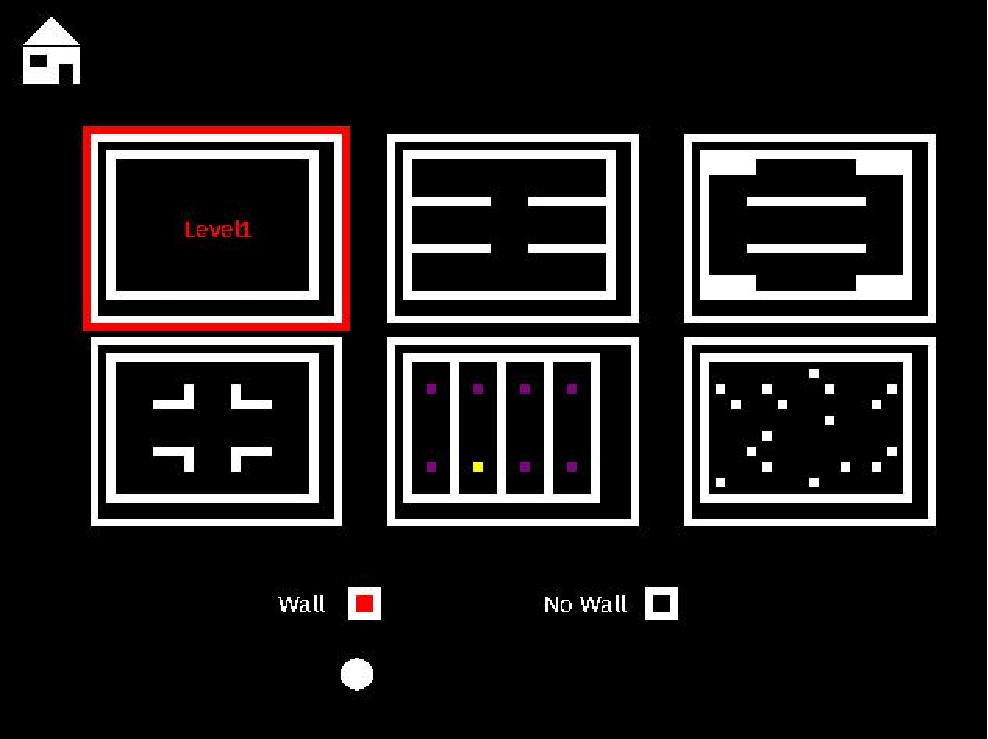
\includegraphics[scale=0.5]{bilder/Einstellungen}
 \captionof{figure}{Einstellungen}
 \label{fig:einstellungen}
\end{minipage}
\newline \\ \\
Wird auf das Zahnrad rechts oben geklickt, {\"o}ffnet sich das Einstellungsmen{\"u} \ref{fig:einstellungen}, indem verschiedene Levels ausgew{\"a}hlt werden k{\"o}nnen und die Au{\ss}enwand aktiviert und deaktiviert werden kann. Ist die Au{\ss}enwand deaktiviert, kann die Schlange beim kollidieren mit der Au{\ss}enwand nicht sterben. Durch klicken auf das Haus links oben kehrt der Spieler zum Hauptmen{\"u} zur{\"u}ck.\newline \newline \\ 
\begin{minipage}[X]{1.1\textwidth}
 \centering
 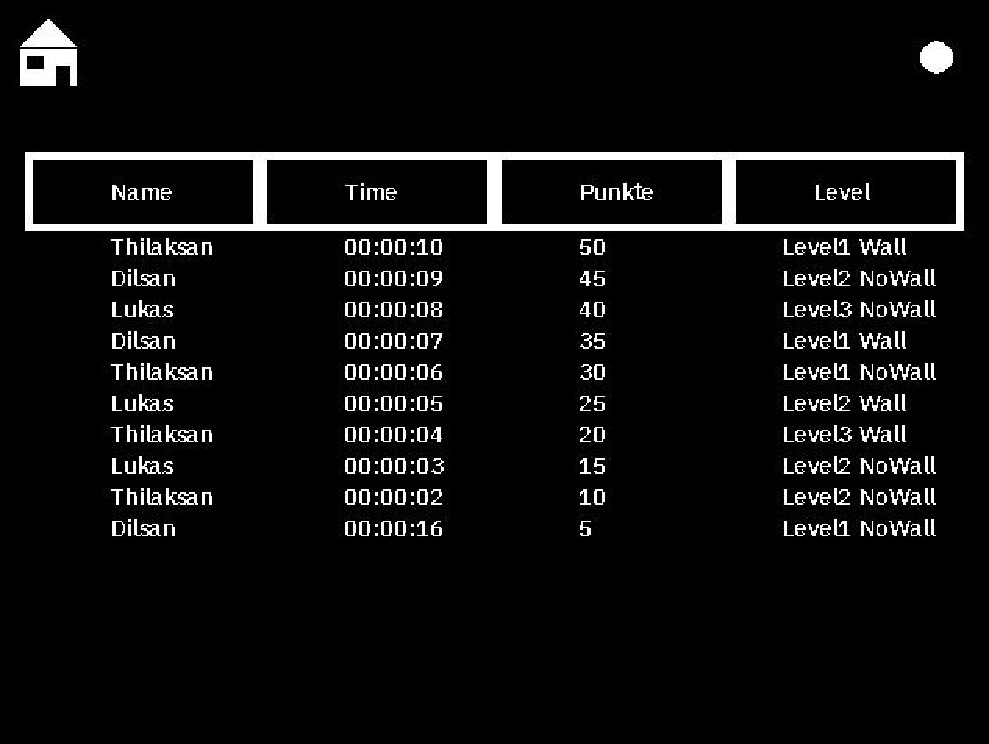
\includegraphics[scale=0.5]{bilder/Highscore}
 \captionof{figure}{Highscore}
 \label{fig:highscore}
\end{minipage}
\newline \\ \\
Wird im Hauptmen{\"u} auf den Highscore-Button geklickt, wird der Highscore \ref{fig:highscore} aus den bisher gespielten Spielen angezeigt. Dabei sind die Highscores prim{\"a}r nach Punkten und sekund{\"a}r nach Zeit sortiert. Au{\ss}erdem steht in jeweils der letzten Zeile der Highscores das Level, indem gespielt wurde. Mit Klicken auf das Haus links oben kehrt der Spieler zur{\"u}ck zum Hauptmen{\"u}.
\\
 Klickt der Spieler auf den \glqq One Player Game\grqq{}-Button {\"o}ffnet sich ein Men{\"u}, indem der Spieler seinen Namen eintragen kann. Dies kann durch Klicken auf die jeweiligen Buttons auf dem Bildschirm oder durch Eingabe {\"u}ber die Tastatur geschehen. Das Spiel wird dann gestartet, wenn der StartGame-Button bet{\"a}tigt wurde. W{\"a}hlt der Spieler den Mehrspielermodus, durch Bet{\"a}tigen des 	\glqq Two Player Game\grqq{}-Button im Hauptmen{\"u}, {\"o}ffnet sich wieder ein Men{\"u} zum Eintragen der Spielernamen und das Spiel kann durch das Bet{\"a}tigen des StartGame-Buttons gestartet werden.  


\section{Spiel - Einzelspielermodus}
\label{Spiel_-_Einzelspielermodus}
%
\begin{figure}[h]
 \centering
 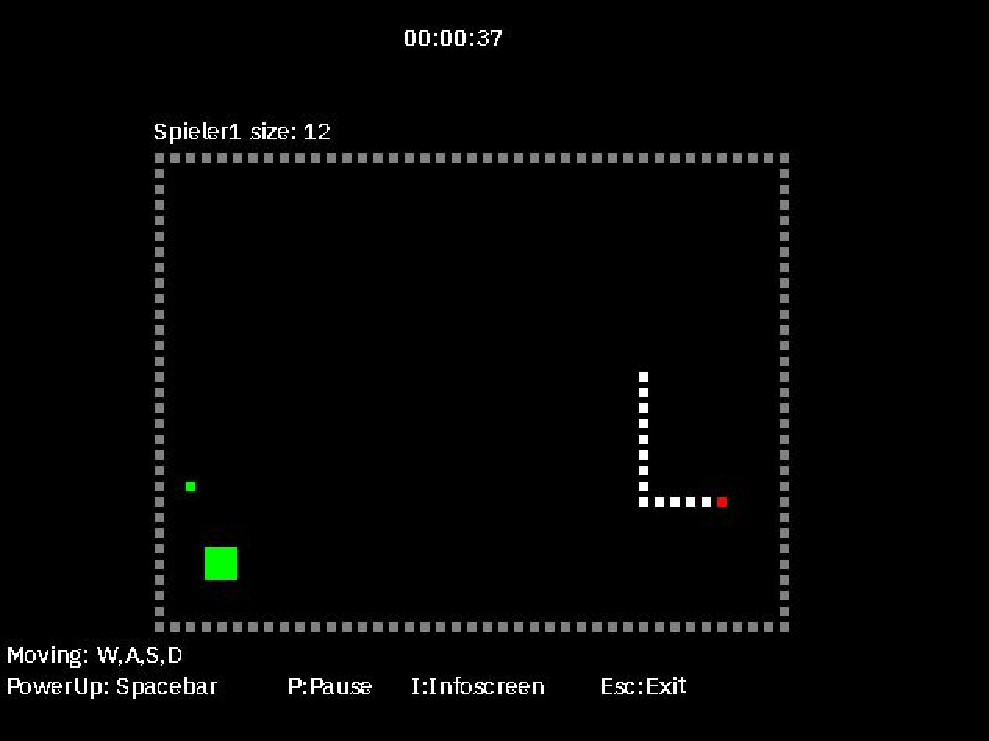
\includegraphics[scale=0.5]{bilder/Einzelspielermodus}
 \caption{Einzelspieler Spiel}
 \label{fig:einzelspielermodus}
\end{figure}
	Der Einzelspielermodus ist im Grunde das traditionelle Snake Game. Die Schlange l{\"a}sst sich steuern durch Bet{\"a}tigen der Tasten W,A,S,D und bewegt sich alle f{\"u}nf Frames. Die gr{\"u}nen Elemente sind das Essen der Schlange, welches die Schlange wachsen l{\"a}sst. Dabei w{\"a}chst die Schlange um eine Gr{\"o}{\ss}e beim Verzehren des kleinen Food-Elements und um zwei beim Verzehren des gro{\ss}en Superfood-Elements.
	Das Spiel kann durch die entsprechenden Levels erschwert werden.Level f{\"u}nf hat ein lilanes Teleport-Element, welches die Schlange zu einem anderen Teleport-Element teleportiert. Dabei teleportieren die oberen Elemente zum n{\"a}chsten rechten Element und die unteren Elemente zum n{\"a}chsten linkem Element. Level 6 ver{\"a}ndert sein inneres Wandmuster nach dem Verzehren des Food-Elements jedoch nicht nach Verzehren des Superfood-Elements. Das Spiel endet, wenn die Schlange mit der Wand oder mit sich selber kollidiert.   


\section{Spiel - Mehrspielermodus}
\label{Spiel_-_Mehrspielermodus}
%
\textcolor{white}{easily}
\newline 
\begin{minipage}[X]{1.0\textwidth}
 \centering
 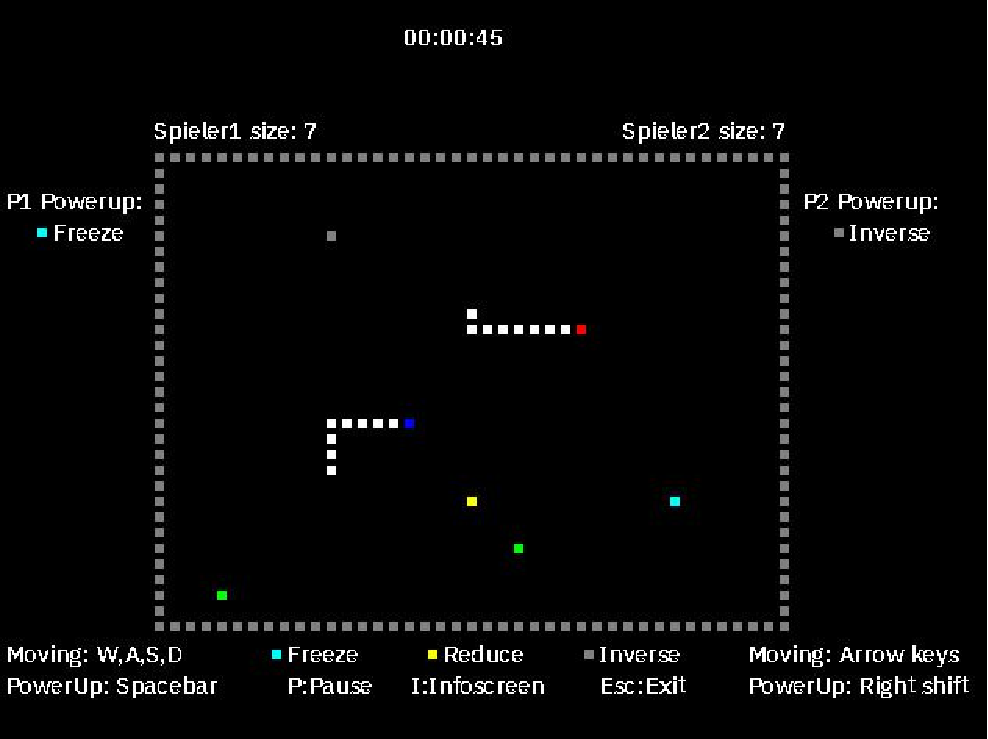
\includegraphics[scale=0.5]{bilder/Mehrspielermodus}
 \captionof{figure}{Mehrspieler Spiel}
 \label{fig:mehrspielermodus}
\end{minipage}
\\ \\ 
	Beim Mehrspielermodus spielen zwei Spieler gegeneinander und versuchen das Spiel durch t{\"o}ten der Schlange des Gegenspielers zu gewinnen. Spieler eins bewegt die rote Schlange mit den Tasten W,A,S,D und Spieler zwei bewegt die blaue Schlange mit den Pfeiltasten. Im Mehrspielermodus gibt es au{\ss}erdem Spezial-Elemente, wie das cyanfarbene Freeze-Element, das gelbe Reduce-Element und das graue Inverse Element. Diese Elemente k{\"o}nnen aufgesammelt werden und mit Leertaste f{\"u}r Spieler eins und mit Shift f{\"u}r Spieler zwei eingesetzt werden. Dabei kann nur ein Element gleichzeitig in der Tasche eines jeweiligen Spielers sein. Beim Einsatz des Freeze-Elementes kann die gegnerische Schlange sich f{\"u}r 25 Frames nicht bewegen. Beim Einsatz des Reduce Elementes veringert sich die L{\"a}nge der gegnerischen Schlange um eine Gr{\"o}{\ss}e. Das Inverse-Element invertiert die Steuerung des Gegenspielers f{\"u}r 250 Frames. Das Spiel ist beendet, wenn eines der Spieler verliert. Kollidiert die Schlange eines Spielers mit der Wand, sich selber oder dem K{\"o}rper der gegnerischen Schlange, verliert derjenige Spieler. Kollidieren beide Schlangen Kopf an Kopf gewinnt derjenige Spieler mit der gr{\"o}{\ss}eren Schlange.  

\section{Spiel - Spielende}
\label{Spiel_-_Spielende}
%
\textcolor{white}{easily}
\newline 
\begin{minipage}[X]{1.1\textwidth}
 \centering
 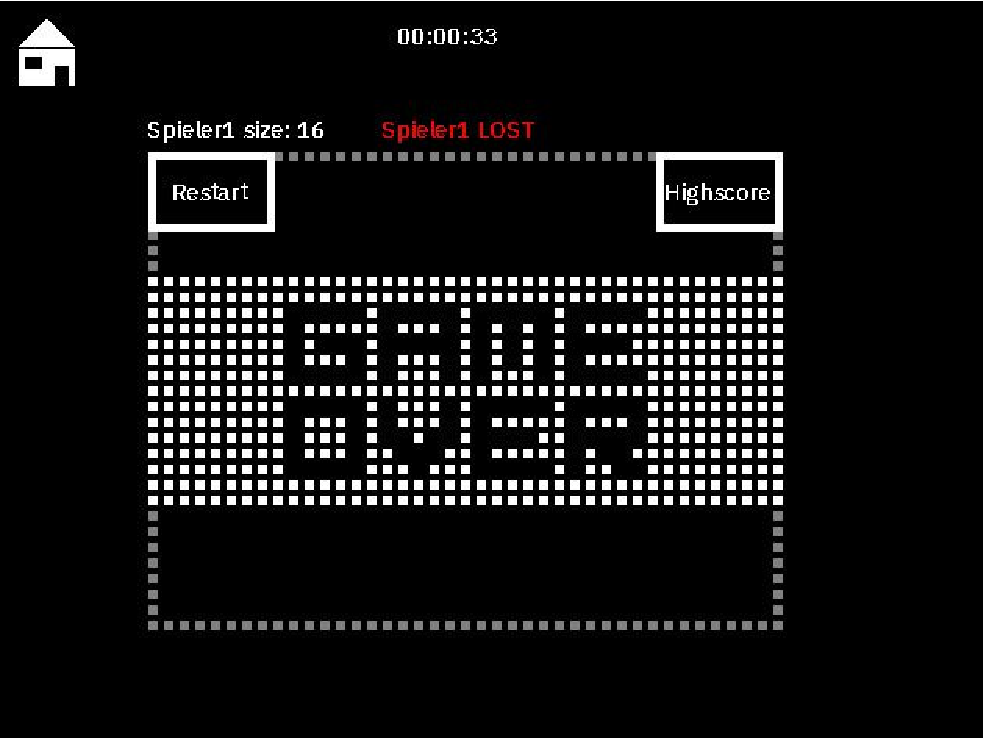
\includegraphics[scale=0.5]{bilder/Spielende}
 \captionof{figure}{Spielende}
 \label{fig:spielende}
\end{minipage}
\\ \\ 
	Ist das Spiel zu Ende erscheint eine kleine Animation und mehrere Buttons. Der Restart-Button startet das Spiel neu und der Highscore-Button zeigt den Highscore an. Au{\ss}erdem steht {\"u}ber dem Spielfeld welcher Spieler gewonnen hat.  

%